\documentclass[openany]{book}
\usepackage[utf8]{inputenc}
\title{Bios * Notes}
\author{Ty Darnell}
\date{ }
\usepackage[english]{babel}
\usepackage [autostyle, english = american]{csquotes}
\MakeOuterQuote{"}
\usepackage{graphicx}
\usepackage{float}
\graphicspath{ {} }
\usepackage{mathtools}
\usepackage{bm}
\usepackage{amsmath, amsthm, amssymb, amsfonts}
\usepackage{caption}
\usepackage{titlepic}
\usepackage{hyperref}
\hypersetup{
	colorlinks=true,
	linkcolor=blue,
	filecolor=magenta,      
	urlcolor=cyan,
	pdftitle={Bios * Notes},
	pdfauthor={Ty Darnell},
	bookmarksopen=true,
}

% For derivatives
\newcommand{\deriv}[1]{\frac{\mathrm{d}}{\mathrm{d}x} (#1)}

% For partial derivatives
\newcommand{\pderiv}[2]{\frac{\partial}{\partial #1} (#2)}

% Integral dx
\newcommand{\dx}{\mathrm{d}x}
\newcommand{\cd}{\overset{d}{\to}}
\newcommand{\cp}{\overset{p}{\to}}
\newcommand{\B}{\beta}
\newcommand{\e}{\epsilon}
\newcommand{\limn}{\lim_{n\to \infty}}
\newcommand{\lm}{\lambda}
\newcommand{\sg}{\sigma}
\newcommand{\hb}{\hat{\beta}}
\newcommand{\sumn}{\sum_{i=1}^{n}}
\newcommand{\hth}{\hat{\theta}}
\newcommand{\bmx}{\bm{X}}
\newcommand{\nxp}{n\times p}
\newcommand{\lra}{\Leftrightarrow}
\newcommand{\bma}{\bm{A}}
\newcommand{\prodn}{\prod_{i=1}^{n}}
\allowdisplaybreaks
\numberwithin{equation}{section}
\newtheorem{proposition}{Proposition}[section]
\begin{document}
	\tableofcontents
\begin{flushleft}
\part{Weisberg}
\chapter{Scatter Plots and Regression}
\chapter{Simple Linear Regression}
\section{Ordinary Least Squares Estimation}
\begin{figure}[H]
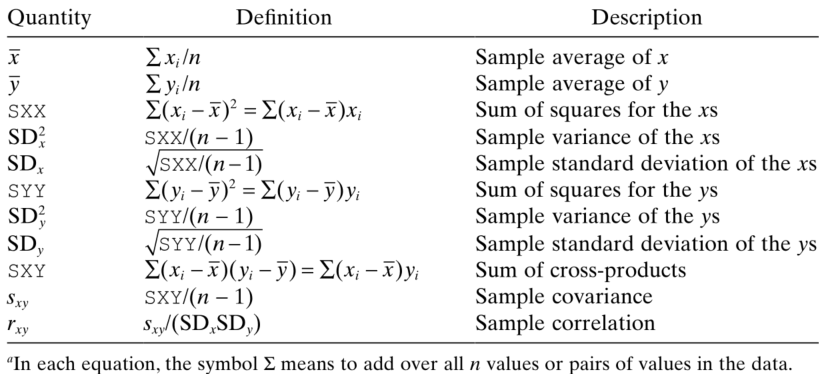
\includegraphics[scale=.6]{olsdefn.png}\\
\end{figure}
Minimize SSR\\
5 Assumptions: HILE Gauss\\
$\hat{\B}_1=\dfrac{SXY}{SXX}=r_{xy}\dfrac{SD_y}{SD_x}=r_{xy}\left(\dfrac{SYY}{SXX}\right)^{1/2}$\\
$\hat{\B}_0=\bar{y}-\hat{\B_1}\bar{x}$
\section{Estimating the Variance}
Residual Mean Square $\hat{\sigma^2}=\dfrac{RSS}{df}$  ($df=n-2$ for SLR)\\
$RSS=SYY-\dfrac{{SXY}^2}{SXX}=SYY-\hat{\B}_1^2SXX$\\
$\hat{sigma^2}\sim \dfrac{\sigma^2}{n-2}\chi^2(n-2)$\\
$\hat{Var}(\hat{\B_1}|X)=\hat{\sigma^2}\dfrac{1}{SXX}$
$\hat{Var}(\hat{\B_0}|X)=\hat{\sigma}^2\left(\dfrac{1}{n}+ \dfrac{\bar{x}^2}{SXX}\right)$\\
$se(\hat{\B_1}|X)=\sqrt{\hat{Var}(\hat{\B_1}|X)}$\\
\section{Confidence Intervals and t-Tests}
\textbf{Intercept}\\
95\% CI:\\
$\hb_0-t(\alpha/2,n-2)se(\hb_0|X)\leq \B_0\leq \hb_0+t(\alpha/2,n-2)se(\hb_0|X)$\\
$H_0:\B_0=B_0^{*} \quad \B_1 \text{ arbitrary}$\\
$H_A:\B_0\neq B_0^{*} \quad \B_1 \text{ arbitrary}$\\
t-statistic $t=\dfrac{\hat{\B}_0-\B_0^{*}}{se(\hat{\B}_0|X)}$\\
\textbf{Slope}:\\
95\% CI:\\
$\hb_1-t(\alpha/2,df)se(\hb_1|X)\leq \B_1\leq \hb_1+t(\alpha/2,df)se(\hb_1|X)$\\
$H_0:\B_1=0$\\
$H_A:\B_1\neq 0$\\
\section{Prediction}
Prediction point of $y_*$  $\tilde{y}_{*}=\hat{\B}_0+\hb_1x_*$\\
$\tilde{y}_{*}$ predicts the yet unobserved $y_*$\\
$y_*=\B_0+\B_1x_*+e_*$\\
$e_*$ is the random error attached to the future value, with variance $\sigma^2$\\
The prediction error variability has second component from
the uncertainty in the estimates of the coefficients.\\
Combining the two sources of variability we have:\\
$Var(\tilde{y}_*|x_*)=\sg^2+\sg^2\left(\dfrac{1}{n}+\dfrac{(x_*-\bar{x})^2}{SXX}\right)$\\
First term is var due to $e_*$ second is error for estimating coefficients\\
$sepred(\tilde{y}_*|x_*)=\sg\left(1+\dfrac{1}{n}+\dfrac{(x_*-\bar{x})^2}{SXX}\right)^{1/2}$\\
A prediction interval uses the t-distribution with df equal to
the df in estimating $\sg^2$\\
\section{Fitted Values}
Obtaining an estimate of $E(Y|X=x_*)$\\
Quantity is estimated by $\hat{y}=\B_0+\B_1x_*$\\
$sefit(\hat{y}|x_*)=\hat{\sg}\left(\dfrac{1}{n}+\dfrac{(x_*-\bar{x})^2}{SXX}\right)^{1/2}$\\
CI:\\
$(\hb_0+\hb_1x)-sefit(\hat{y}|x)[2F(\alpha;2,n-2)]^{1/2}\leq y\leq (\hb_0+\hb_1)+sefit(\hat{y}|x)[2F(\alpha;2,n-2)]^{1/2}$\\
\section{Coefficient of Determination}
$SYY$ Total sum of squares\\
$SSreg=SYY-RSS$\\
$SSreg=SYY-\left(SYY-\dfrac{(SYY)^2}{SXX}\right)=\dfrac{(SXY)^2}{SXX}$\\
$R^2=\dfrac{SSreg}{SYY}=1-\dfrac{RSS}{SYY}$\medbreak
The left side is the proportion of variability in the response explained by regression on the predictor. The right side is 1 minus the remaining unexplained variability.
\begin{itemize}
\item $R^2$ is a scale-free one-number summary of the strength of the relationship
between the $x_i$ and the $y_i$ in the data.\\
\item Interpret as: about $R^2$\% of the variablity in the observed values of the model are explained by the predictor variable.\\
\item In SLR $R^2$ is the same as the square of the sample correlation between predictor and response\\
\end{itemize}
$R_{adj}^2=1-\dfrac{RSS/df}{SYY/(n-1)}$\\
adding a correction for df of the sums of squares that can facilitate comparing models in multiple regression
\section{Residuals}
Most common plot in SLR is resid vs fitted values
\begin{itemize}
\item A null plot would indicate no failure
of assumptions\\
\item Curvature might indicate that the fitted mean function is inappropriate\\
\item Residuals that seem to increase or decrease in average magnitude with the fitted values might indicate nonconstant residual variance\\
\item A few relatively large residuals may be indicative of outliers, cases for which the model is somehow inappropriate.
\end{itemize}
\chapter{Multiple Regression}
\section{Adding a Regressor to an SLR Model}
Start with $E(Y|X_1=x_1)=\B_0+\B_1x_1$\\
adding $X_2$ $E(Y|X_1=x_1,X_2=x_2)=\B_0+\B_1x_1+\B_2x_2$\\
The main idea in adding $X_2$ is to explain the part of Y that has not already been explained by $X_1$\\
\section{The MLR Model}
$E(Y|X)=\B_0+\B_1X_1+\cdots+\B_pX_p$ Conditioning on all regressors on the right side\\
$E(Y|X=x)=\B_0+\B_1X_1+\cdots+\B_pX_p$ Conditioning on specific values for the predictors\\
When the number of regressors, $p=2$ the mean function corresponds to a plane in  
3 dimensions\\
When $p>2$, the fitted mean function is a hyperplane\\
\section{Predictors and Regressors}
\begin{itemize}
\item \textbf{Predictors}- the simplest type of regressor is equal to a predictor\\
\item \textbf{Transformations of predictors}- sometimes original predictors need to be transformed to make the general MLR model hold to a reasonable approximation\\
\item \textbf{Polynomials}- Problems with curved mean functions can sometimes be accommodated in the MLR model by including polynomial regressors in the predictor variables. Could include both a predictor $X_1$ and its square $X_1^2$ to fit a quadratic polynomial in that predictor.\\
\item \textbf{Interactions and other combinations of predictors}- Combining several predictors is often useful. ex: bmi which is a function of both weight and height in place of both height and weight.\\
\item \textbf{Interactions}- Products of regressors are often included in a mean function along with the base regressors to allow for joint effects.\\
\item \textbf{Factors}- A categorical predictor with two or more
levels. Factors are included in MLR using \textbf{dummy variables} which are typically regressors that have only two values, 0 and 1 indicating which category is present for a particular observation.\\
\end{itemize}
The marginal relationships between the response and each of the variables is not sufficient to understand the joint relationship between the response and the regressors.\\
The interrelationships among the regressors are also important.\\
The pairwise relationships between the regressors can be viewed in the remaining cells of the scatterplot matrix.\\
A more traditional, and less informative, summary of the two-variable
relationships is the matrix of sample correlations.\\
\section{Ordinary Least Squares}
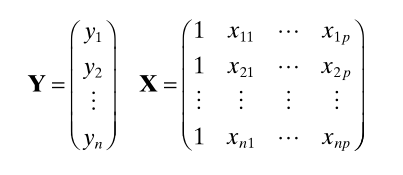
\includegraphics[scale=.7]{matnot.png}\\
$\boldsymbol{\B}=(\B_0,\B_1,\dots,\B_p)^{'}$  $(p+1)\times1$ vector of unknown regression coefficients\\
Equation for the mean function evaluated at $\bm{x}_i$ is:\\ $E(Y|X=\boldsymbol{x}_i)=\boldsymbol{x}_i^{'}\bm{\B}$\\
Mean function in matrix terms:\\
$E(\bm{Y}|\bm{X})=\bm{X}\bm{\B}$\\
$\bm{Y}$ is vector of responses, $\bm{X}$ is the $nx(p+1)$ matrix whose $ith$ row is $\bm{x}_i^{'}$
\subsection{The Errors e}
Define the unobservable random vector of errors $\bm{e}$ elementwise by:\\
$e_i=y_i=E(Y|X=\bm{x}_i)=y_i-\bm{x}_i^{'}\bm{\B}$\\
$\bm{e}=(e_i,\dots,e_n)^{'}$\\
$E(\bm{e}|X)=0 \quad Var(\bm{e}|X)=\sg^2\bm{I}_n$\\
where $Var(e|X)$ means the covariance matrix of $\bm{e}$ for a fixed value of X, $\bm{I}_n$ is the $nxn$ matrix with ones on the diagonal and zeroes everywhere else.\\
Adding the assumption of normality we can write:\\
$(\bm{e}|X)\sim N(\bm{0},\sg^2\bm{I}_n)$\\
\subsection{OLS Estimators}
The least squares estimate $\bm{\hb}$ of $\bm{\B}$ is chosen to minimize the residual sum of squares function:\\
\[RSS(\bm{\B})=\bm{\sum}(y_i-\bm{x}_i^{'})^2=(\bm{Y}-\bm{X\B})^{'}(\bm{Y}-\bm{X\B})\]\\
OLS estimate $\bm{\hb}=(\bm{X^{'}X})^{-1}\bm{X^{'}Y}$ provided the inverse $\bm{X^{'}X}^{-1}$ exists\\
Do not use the above equation to compute least squares estimates because of potential rounding errors\\
$\bm{\hb}$ depends only on the sufficient statistics $\bm{X^{'}X}$ and $\bm{X^{'}Y}$ which are matrices of uncorrected sums of squares and cross products.\\
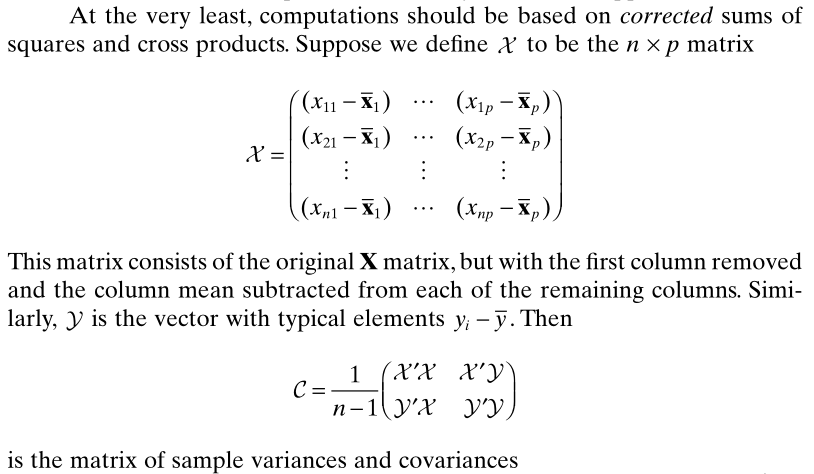
\includegraphics[scale=.6]{covmat.png}\\
\part{Class Notes}
\chapter{Notes 2 Matrix Algebra}
\textbf{Symmetric Matrix}- $\bm{A}$ where $a_{ij}=a_{ji} \quad \forall \ i,j$\\
\textbf{Trace}- sum of diagonal elements of a square matrix\\
\textbf{Matrix Multiplication} $\bm{A}_{r\times s}\bm{B}_{s\times t}=\left\{\sum_{k=1}^{s}a_{ik}b_{kj} \right\}=\bm{C}_{r\times t}$\\
\section{Orthogonal}
\text{Orthogonal Matrix}- a square matrix with $\bm{A^{'}}=\bm{A^{-1}}$\\
A square matrix $\bm{A}$ is orthogonal if $\bm{A^{'}A}=\bm{I}=\bm{AA^{'}}$\\
Two vectors x and y are orthogonal if $x^{'}y=0$\\
x and y are \textbf{orthonormal} if they are orthogonal and are normalized: $x^{'}y=0$ , $x^{'}x=1$, $y^{'}y=1$\\
An orthogonal matrix has orthonormal columns.\\
\section{Rules of Matrix Operation}
\textbf{Distributive Laws}\\
\begin{itemize}
\item $A(B+C)=AB+AC$
\item $(B+C)D=BD+CD$
\end{itemize}
\textbf{Associative Laws}\\
$(AB)C=A(BC)$
\textbf{Transpose Operations}\\
\begin{itemize}
\item $(A+B)^{'}=A^{'}+B^{'}$
\item $(AB)^{'}=B^{'}A^{'}$
\end{itemize}
\section{Linear Dependence and Rank}
The columns of $\bm{A}$ are \textbf{linearly dependent} if they contain redundant information\\
If we can find two distinct vectors $\lambda$ and $\gamma$
such that $\bm{A\lm}=\bm{A\gamma}=\bm{x}$ then the columns of $\bm{A}$ are linearly dependent\\
Equivalently let $\delta=\lm-\gamma$\\
The columns of $\bm{A}$ are linearly dependent if there exists a vector $\delta\neq 0$ such that $\bm{A\delta}=\bm{0}$\\
\textbf{Rank} of $\bm{A}$ is the number of linearly independent columns in $\bm{A}$\\
If $\bm{A}$ is an $(r\times c)$ matrix with $r\geq c$, $\bm{A}$ is \textbf{full rank} if $rank(\bm{A})=c$\\
If $rank(\bm{A})<c$ $\bma$ is less than full rank\\
In linear regression, the matrix of covariates $\bmx$ must have full rank in order for the parameter estimates $\bm{\hb}$ to be unique\\
A square matrix less than full rank is called \textbf{singular}, if full rank called \textbf{nonsingular}\\
\textbf{Elementary Row Operations}:
\begin{enumerate}
\item multiplying a row by a nonzero constant
\item adding one row to another
\item exchanging two rows
\end{enumerate}
\section{Determinants}
\textbf{Determinant}- a single number summary of a square matrix that gives us information about the rank of the matrix\\
The determinant of a diagonal or triangular matrix is the product of the diagonal values\\
If determinant=0 then the matrix is less than full rank and the inverse does not exist\\
If $det\neq 0$ then the inverse exists and full rank\\
For full rank matrices that conform, $|\bm{AB}|=|\bma||\bm{B}|$\\
Also $|\bma^{'}|=|\bma|$
\section{Positive Definite and Semidefinite Matrices}
Let $\bma$ be an $n\times n$ symmetric matrix. $\bma$
is \textbf{positive definite} iff:
\begin{enumerate}
\item $a_{ii}>0 \quad \forall \ i=1,\dots,n$
\item The determinant of every square submatrix of upper-left corner of $\bma$ is positive
\end{enumerate}
\textbf{Positive semidefinite} if we replace $>0$ with $\geq 0$\\
\textbf{Nonnegative definite}- positive definite or positive semidefinite\\
Covariance matrices are nonnegative definite\\
\section{Inverses}
\textbf{Normal equations} for the linear model:\\
$(\bmx_{n\times p})^{'}(\bmx_{n \times p})\bm{\hb}=(\bmx_{n\times p})^{'}\bm{y}_{n\times 1}$\\
If $\bma$ is full rank then there exists a unique matrix $\bma^{-1}$, the inverse of $\bma$ where:\\
$\bma^{-1}\bma=\bma\bma^{-1}=\bm{I}$\\
\textbf{Properties of Inverses}\\
\begin{enumerate}
\item For a scalar $\bma_{1\times 1} =a, \ \bma^{-1}=\dfrac{1}{a}$
\item The inverse of a diagonal matrix is the diagonal matrix of reciprocals of the diagonal elements
\item For conforming full rank matrices, $(\bm{AB})^{-1}=\bm{B}^{-1}\bma^{-1}$
\item A symmetric matrix has a symmetric inverse
\item $(\bma^{'})^{-1}=(A^{-1})^{'}$
\item The determinant of the inverse is the inverse of the determinant. $|\bma^{-1}|=\dfrac{1}{|\bma|}$
\item Inverse of a $2\times 2$ matrix
 \[\bma=
\left( \begin{array}{cc}
a_{11}& a_{12}\\
a_{21}&a_{22}
\end{array}\right)
\]
\[\bma^{-1}=\dfrac{1}{|\bma|}\left(\begin{array}{cc}
a_{22}&-a_{12}\\
-a_{21}& a_{11}
\end{array}\right)
\]
\end{enumerate}
\section{Eigenvalues and Eigenvectors}
\textbf{Eigenanalysis} is defined only for square matrices\\
$\bm{A}$ is an $n\times n$ matrix\\
\textbf{Right eigenvector} of $\bma$ is any nonzero $n\times 1$ vector $x$ satisfying $\bm{Ax}=\lambda\bm{x}$\\
$\lm$ is the \textbf{eigenvalue} corresponding to x\\
eigen is German for characteristic\\
Eigenvectors are not unique, convention is to scale the eigenvector x so that $x^{'}x=1$, normalizing it to unit length\\
\pagebreak
\section{Finding Eigenvectors and Eigenvalues}
An $n\times n$ matrix has n eigenvalues\\
Definition of eigenvectors: $\bma\bm{x}=\lm\bm{x}$\\
Characteristic equation: $|\bma-\lm\bm{I}|=\bm{0}$\\
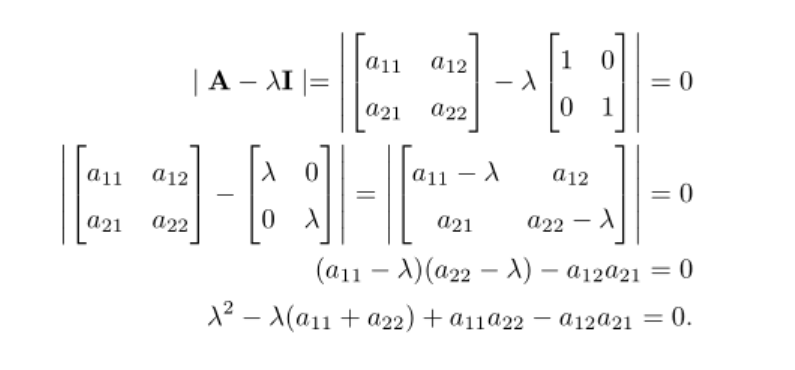
\includegraphics[scale=.5]{eigen.png}\\
eigenvectors corresponding to these eigenvalues can be found using the equation $\bm{Ax}=\lm\bm{x}$\\
Normalize an eigenvector $x=(x_1,x_2)^{'}$: $\dfrac{1}{\sqrt{x_1^2+x_2^2}}(x_1,x_2)^{'}$\\
\section{Properties of Eigenvalues and Eigenvectors}
\begin{itemize}
\item For $\bma_{n\times n}$ number of distinct eigenvalues ranges from 1 to n
\item $trace(\bma)=\sum_{i=1}^{n}\lm_i$
\item $|\bma|=\prod_{i=1}^{n}\lm_i$
\item $\bma$ full rank $\lra \bma$ has no zero eigenvalues
\item  $|\bma|=0\lra$ at least one eigenvalue is zero $\lra \bma$ is not full rank
\item The number of nonzero eigenvalues of $\bma$ is $rank(\bma)$
\item Small eigenvalues imply that there are near-linear dependencies in the columns of $\bma$
\item $\bma$ is positive definite if $min(\lm_i)>0$
\item $\bma$ is positive semidefinite if $min(\lm_i)\geq 0$
\end{itemize}
\section{Random Vectors and Matrices}
$\bm{Z}$ is an $(n\times p)$ matrix of random variables
\[E(\bm{Z})=\left(
\begin{array}{ccc}
E(Z_{11})&\dots&E(Z_{1p})\\
\vdots & \dots & \vdots\\
E(Z_{n1}) &\dots& E(Z_{np})
\end{array}
\right)
\]
The expectation of a random matrix is the matrix of the
expectations\\
For $\bm{Y}$ an $(n\times 1)$ random vector, the \textbf{covariance matrix} is:
\begin{multline*}\\
Cov(\bm{Y})=E[(\bm{Y}-\bm{\mu})(\bm{Y}-\bm{\mu})^{'}]\\
=\bm{\Sigma}=\left(
\begin{array}{cccc}
\sigma_{11}&\sigma_{12}&\cdots& \sg_{1n}\\
\sg_{21}& \vdots & \vdots & \vdots\\
\vdots & \vdots & \vdots & \vdots\\
\sg_{n1} &\cdots & \cdots& \sg_{nn} 
\end{array}
\right)\\
\text{where } \sg_{ij}=E[(Y_i-\mu_i)(Y_j-\mu_j)^{'}] \quad i,j=1,\dots,n\\
\end{multline*}
\text{Let } $\bm{\mu}=E(\bm{Y})$ and $\bm{\Sigma}=Cov(\bm{Y})$\\
Suppose $\bma_{r\times n}$ is a matrix of constants and $\bm{b}_{r \times 1}$ is a vector of constants. Then:\\
$E(\bm{AY}+\bm{b})=\bma E(\bm{Y})+\bm{b}=\bm{A\mu}+\bm{b}$\\
$Cov(\bm{AY}+\bm{b})=\bma Cov(\bm{Y})\bma^{'}=\bma\bm{\Sigma}\bma^{'}$
Let $\bm{W}_{r\times 1}$ be a random vector with $E(\bm{W})=\bm{\gamma}$ Then:\\
$Cov(\bm{W},\bm{Y})=E[(\bm{W}-\bm{\gamma})(\bm{Y}-\bm{\mu})^{'}]$\\
Where $Cov(\bm{W},\bm{Y})$ is an $(r\times n)$ matrix of covariances with $ij^{th}$ element equal to $Cov(W_i,Y_j)$\\
\section{Multivariate Normal Distribution}
Suppose $X=(X_1,\dots,X_n)^{'}$ Then X has an $n$ dimensional multivariate normal distribution with mean $\mu$ and covariance matrix $\Sigma$ if X has density:
\[f(x)=\dfrac{1}{(2\pi)^{n/2}|\Sigma|^{1/2}}\exp\left\{-\dfrac{1}{2}(x-\mu)^{'}\Sigma^{-1}(x-\mu) \right\}
\]
$X\sim N_n(\mu,\Sigma)$\\
$\Sigma$ must be positive definite\\
\section{Facts about the multivariate normal distribution}
\begin{enumerate}
\item A linear transformation of a multivariate normal distribution (mvn) yields another mvn.\\
If $X\sim N_n(\mu,\Sigma)$ and $Y=AX+b$\\
with $\bma_{r\times n}$  matrix of constants and $\bm{b}_{r \times 1}$ vector of constants.\\
Then $Y\sim N_r(A\mu+b,A\Sigma A^{'})$\\
\item A linear combination of independent mvn distributions is an mvn distribution.\\
Suppose $X_1,\dots,X_k$ are independent with $X_i\sim N_n(\mu_i,\Sigma_i)\quad i=1,\dots,k$ and\\
$a_1,\dots,a_k$ are scalars\\
Define $Y=a_1X_1+\dots+a_kX_k$\\
Then $Y\sim N(\mu^*,\Sigma^*)$ where $\mu^{*}=\sum_{i=1}^{k}a_i\mu_i$ and $\Sigma^*=\sum_{i=1}^{k}a_i^2\Sigma_i$
\item Marginal distributions of mvn are also mvn\\
Suppose $X\sim N_n(\mu,\Sigma)$\\
Partition X into $X={X_1\choose X_2}$ where $X_1$ is $r\times 1$ and $X_2$ is $(n-r)\times 1$\\
Partition $\mu$ as $\mu={\mu_1\choose \mu_2}$ where $\mu_1$ is $r\times 1$ and $\mu_2$ is $(n-r)\times 1$\\
Partition $\Sigma$ as:
\[\Sigma=\left(
\begin{array}{cc}
\Sigma_{11}&\Sigma_{12}\\
\Sigma_{21}&\Sigma_{22}
\end{array}
\right)
\]
where $\Sigma_{11}$ is $r\times r$, $\Sigma_{21}$ is $(n-r)\times r$ and $\Sigma_{22}$ is $(n-r)\times (n-r)$\\
Then marginal distribution of $X_1\sim N_r(\mu_1,\Sigma_{11})$\\ 
Marginal distribution of $X_2\sim N_{(n-r)}(\mu_2,\Sigma_{22})$
\item Conditional distributions of mvn are mvn.\\
Suppose $X\sim N_n(\mu,\Sigma)$\\
Using same partition as above, we have:\\
$X_1|X_2=x_2\sim N_r(\mu_1+\Sigma_{12}\Sigma_{22}^{-1}(x_2-\mu_2),\Sigma^*)$\\
where $\Sigma^*=\Sigma_{11}-\Sigma_{12}\Sigma_{22}^{-1}\Sigma_{21}$\\
\end{enumerate}
\chapter{GLM Estimation and Testing}
\begin{multline*}\\
\bm{\hb}=\bm{(X^{'}X)^{-1}X^{'}y}\text{ if X is full rank}\\
\bm{H}=\bm{X(X^{'}X)^{-1}X^{'}} \text{ hat matrix, same rank as X}\\
\hat{\bm{y}}=\bm{X\hb}=\bm{Hy} \text{ predicted values}\\
\bm{\hat{\epsilon}}=\bm{y-\hat{y}}=\bm{y-Hy}=\bm{(1-Hy)}\\
\end{multline*}
\section{GLH}
assume iid Gaussian errors.\\
$\bm{\B}$ is the matrix of primary parameters\\
$\bm{\theta}_{ax1}=\bm{C}_{axp}\bm{\B}_{px1}$ is a matrix of secondary parameters defined by $\bm{C}$\\
Each row of $\bm{C}$ defines a new scalar parameter in terms of the $\bm{\B}$'s ex: $\B_1-\B_2$\\
Let $\bm{\theta}_0$ be matrix of known constants (hypothesized values) usually zero matrix\\
\begin{center}
\textbf{The (Univariate) General Linear Hypothesis:}\\
$H_0:\bm{\theta}_{ax1}=\bm{\theta}_0$\\
$H_A:\bm{\theta}_{ax1}\neq\bm{\theta}_0$
\end{center}
\pagebreak
\section{Estimability of a Parameter}
A (linear) function of the parameters is
defined to be \textbf{estimable} if it is identically equal to some linear function of the expected value of the vector of observations, $\bm{y}$\\
\begin{itemize}
\item A scalar parameter,
$\theta_i=\bm{C}_{1xp}\bm{\B}_{px1}$ is estimable $\lra \bm{C}_{1xp}\bm{\B}_{px1}=\bm{t^{'}}_{1xn}E(\bm{y}_{nx1})$\\
for $\bm{t}$ a vector of constants
\item For a vector we need:
$\bm{\theta}_{ax1}=\bm{T}_{axn}E(\bm{y}_{nx1})$\\
\end{itemize}
There always exists $r=rank(\bm{X})$ distinct and estimable parameters\\
These are not necessarily elements of $\bm{\B}$ but may be linear combinations of elements
\begin{itemize}
\item If $rank(\bm{X})=r=p$, then $\bm{\hb}$ exists (uniquely), 
$\bm{\B}$ is estimable and any (nonzero) $\bm{C}$ gives estimable $\bm{\theta}$\\
This is usually the case with continuous predictors unless some predictors are collinear
\item  If $rank(\bm{X})=r<p$, $\bm{\B}$ is not estimable (although as many as $r$ elements may be), and for $\bm{\hat{\theta}}=\bm{C\B}$, we must check estimability.
\end{itemize}
To show a set of parameters:
$\bm{\theta}_{a\times 1}=\bm{C}_{a\times p}\bm{\B}_{p\times1}=\bm{T}_{a\times n}E(\bm{y}_{n\times 1})$ is estimable:\\
show that $\bm{C}_{a\times p}=\bm{T}_{a\times n}\bm{X}_{n \times p}$\\
Estimable $\bm{\hat{\theta}}$ shares the optimality of $\bm{\hb}$\\
\section{Testability of a Hypothesis}
\textbf{Likelihood Ratio (LR) Test} - used for comparing the goodness of fit of two statistical models (null and alternative)\\
The test is based on the \textbf{likelihood ratio}, which expresses how many times more likely the data are under one model than the other.\medbreak
Let $\bm{M}_{a\times a}=\bm{C(X^{'}X)^{-1}C^{'}}$\\
Define GLH testability as the (unique) existence of the LR test\\
$\bm{\theta}$ is testable $\lra$
\begin{itemize}
\item $\bm{C}$ is full rank $a$ (no redundancies) and
\item $\bm{\theta}$ is estimable\\
\end{itemize}
Or equivalently
\begin{itemize}
\item $\bm{M}$ is full rank $a$ and
\item $\bm{\theta}$ is estimable
\end{itemize} 
If $\bm{X}$ is full rank then $\bm{\theta}$ is testable $\Leftrightarrow$\\
$\bm{C}$ is full rank $a$ or $\bm{M}$ is full rank a (because any $\bm{\theta}$ is estimable)\\
\section{Computation of Test Statistic and p-value}
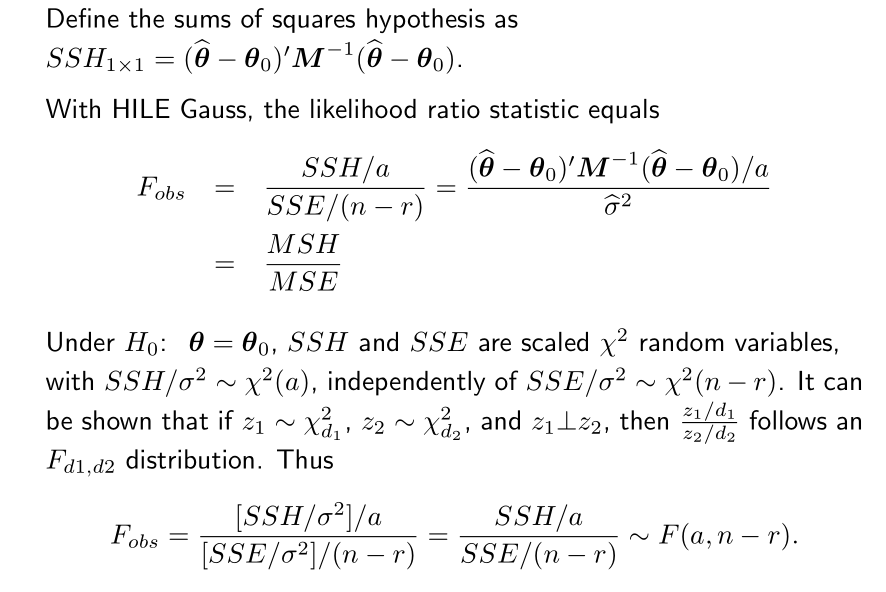
\includegraphics[scale=.5]{lr.png}\\
The p-value equals the probability of observed or more extreme data
arising under the null:\\
p-value$=P\{F(a,n-r)\geq F_{obs} \}=1-P\{F(a,n-r)<F_{obs} \}$\\
Reject $H_0$ if $F_{obs}>f_{crit}=F^{-1}(1-\alpha,a,n-r)$\\
$qf(prob,{df}_1,{df}_2)$ (F statistic)\\
$1-pf(crit,{df}_1,{df}_2)$ (p-value)\medbreak
All linear model GLH tests correspond to comparing two models, the
"full" model, $\bm{y}=\bm{X\B}+\bm{\epsilon}$ and a reduced model defined by
constraints
\section{Wald Tests}
For a single coefficient $\B_j$ we can test $H_0:\B_j=0$ if $\B_j$ is estimable\\
Using properties of the standard normal distribution we can base our test on the ratio:
\[t=\dfrac{\hb_j-0}{\sqrt{var(\hb_j)}}
\]
Obtain estimate $\hat{\sg}^2=\dfrac{SSE}{dfE}$\\
If we know $\sigma^2$ exactly then $t\sim N(0,1)$\\
If we estimate $\sg^2$ from the data then $t\sim t_{dfE}$\\
\section{F-Tests}
two-sided F test uses $\alpha$ critical value\\
one-sided F test uses $2\alpha$ critical value\\
\chapter{Some Distributional Results for the GLM}
In analysis with the GLM, we use three kinds of distributions:
multivariate Gaussian, $\chi^2$ and $F$\\
Assume HILE Gauss assumptions hold
\section{A Full Rank Basis For Less Than Full Rank Models}
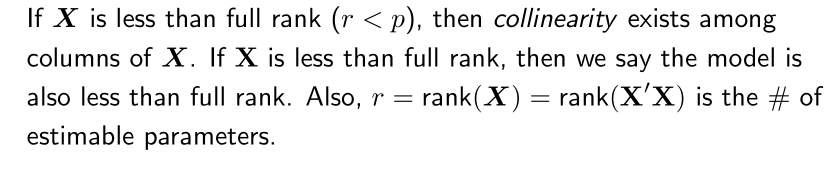
\includegraphics[scale=.5]{col.png}\\
For every less than full rank model, there exists a corresponding full rank model with $r$ estimable parameters.\\
That is: for less than full rank $\bm{X}$ there exists a $p\times r$ matrix $\bm{V}_{+}$ such that:\\
$\bm{X}_{n\times p}=\bm{X}_{*,(n\times r)}\bm{V^{'}}_{+,(r\times p)}$\\
with $rank(\bm{X}_*)=rank(\bm{V_{+}})=r<p$\\
$\bmx_*$ provides a \textbf{full rank basis} for $\bmx$\\
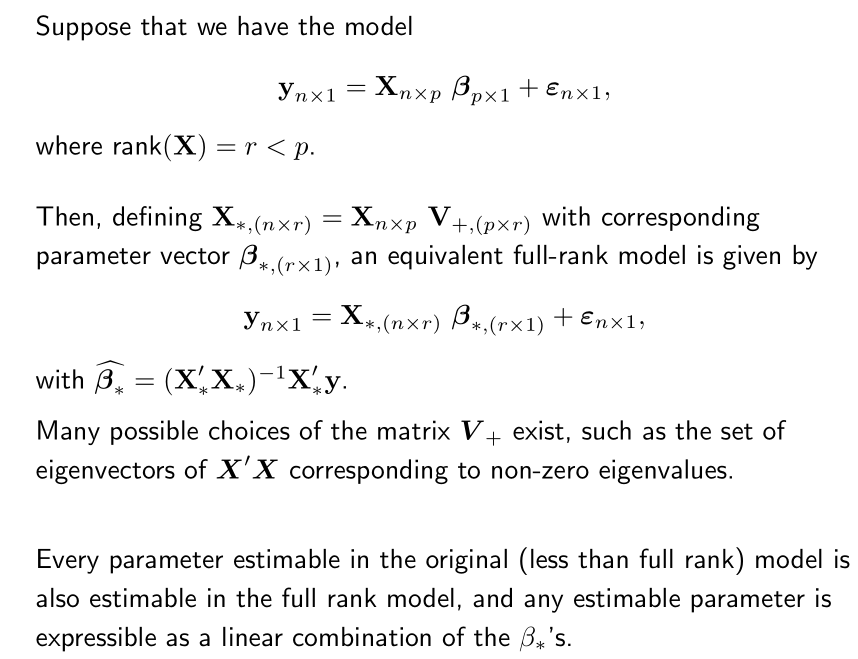
\includegraphics[scale=.5]{frb.png}\\
\chapter{Multiple Regression General Consideration}
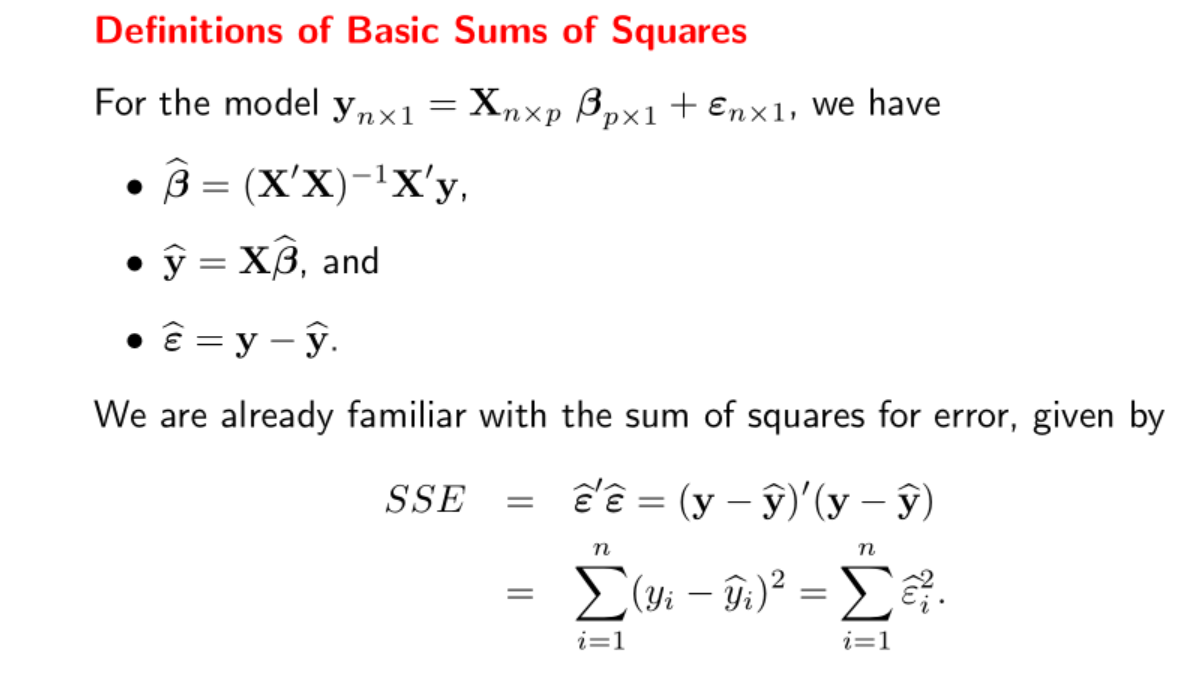
\includegraphics[scale=.55]{ss.png}\\
\end{flushleft}
\end{document}
